\documentclass[10pt]{article}

% ---------- Page / geometry ----------
\usepackage[a4paper,margin=13mm,top=11mm,bottom=14mm]{geometry}
\usepackage[T1]{fontenc}
\usepackage[utf8]{inputenc}
\usepackage{textcomp}
\usepackage{helvet}
\renewcommand{\familydefault}{\sfdefault}

% ---------- Color / graphics ----------
\usepackage[table]{xcolor}
\usepackage{tikz}
\usepackage{tabularx}
\usepackage{array}
\usepackage{booktabs}
\usepackage{colortbl}
\usepackage{enumitem}
\usepackage{fancyhdr}
\usepackage{amssymb}
\usepackage{ragged2e}

% ---------- Palette ----------
\definecolor{ink}{HTML}{15181C}
\definecolor{rulegrey}{HTML}{C9CFD6}
\definecolor{lightgrey}{HTML}{F2F4F7}
\definecolor{warnred}{HTML}{B5271B}
\definecolor{warnbg}{HTML}{FBE6E3}

% Phase accent colors:  P1 BLUE  /  P2 GREEN  /  P3 ORANGE
\definecolor{p1}{HTML}{1D5FA8}  \definecolor{p1bg}{HTML}{E7F0FA}
\definecolor{p2}{HTML}{1E8449}  \definecolor{p2bg}{HTML}{E6F4EC}
\definecolor{p3}{HTML}{C9620A}  \definecolor{p3bg}{HTML}{FCEFE0}

% Filament / info accents
\definecolor{infobg}{HTML}{EEF1F5}
\definecolor{infohd}{HTML}{2C3540}

% ---------- Header / footer ----------
\pagestyle{fancy}
\fancyhf{}
\renewcommand{\headrulewidth}{0pt}
\renewcommand{\footrulewidth}{0.4pt}
\renewcommand{\footrule}{\hbox to\headwidth{\color{rulegrey}\leaders\hrule height \footrulewidth\hfill}}
\fancyfoot[L]{\footnotesize\color{ink!60}InMoov Right Hand + Forearm --- 3-Phase Print Checklist}
\fancyfoot[R]{\footnotesize\color{ink!60}Page \thepage}
\setlength{\headheight}{12pt}

\setlength{\parindent}{0pt}
\setlength{\tabcolsep}{3.5pt}
\renewcommand{\arraystretch}{1.28}

% ---------- Checkbox ----------
\newcommand{\cbox}{\tikz[baseline=-0.15ex]\draw[line width=0.6pt,rulegrey!150,fill=white] (0,0) rectangle (3.6mm,3.6mm);}

% ---------- Inline warning ----------
\newcommand{\wlab}{\textcolor{warnred}{\bfseries$\triangle$\,WARNING:}}
\newcommand{\tlab}{\textbf{TIP:}}
\newcommand{\nlab}{\textbf{Note:}}

% ---------- Column types ----------
\newcolumntype{K}{>{\centering\arraybackslash}m{8mm}}
\newcolumntype{P}{>{\centering\arraybackslash}m{14mm}}
\newcolumntype{Q}{>{\centering\arraybackslash}m{10mm}}
\newcolumntype{W}{>{\centering\arraybackslash}m{11mm}}
\newcolumntype{S}{>{\centering\arraybackslash}m{13mm}}
\newcolumntype{R}{>{\centering\arraybackslash}m{17mm}}

% ---------- Table header row ----------
\newcommand{\thead}[1]{%
\rowcolor{#1}
{\color{white}\bfseries Done} & {\color{white}\bfseries\ STL part file} & {\color{white}\bfseries Layer} & {\color{white}\bfseries Infill} & {\color{white}\bfseries Walls} & {\color{white}\bfseries Supp.} & {\color{white}\bfseries Raft}\\}

% ---------- Part settings row ----------
% #1 number  #2 filename  #3 layer  #4 infill  #5 walls  #6 support  #7 raft
\newcommand{\prow}[7]{%
\cbox & {\bfseries #1.}\,\texttt{\small #2} & #3 & #4 & #5 & #6 & #7\\}

% ---------- Full-width note / warning rows (span all 7 columns) ----------
\newcommand{\pnote}[1]{%
\rowcolor{lightgrey}\multicolumn{7}{p{\dimexpr\textwidth-2\tabcolsep\relax}}{\footnotesize #1}\\}
\newcommand{\pwarn}[1]{%
\rowcolor{warnbg}\multicolumn{7}{p{\dimexpr\textwidth-2\tabcolsep\relax}}{\footnotesize\wlab\ \textcolor{warnred}{#1}}\\}

% ---------- Phase header bar ----------
% #1 accent  #2 bg  #3 title  #4 tag  #5 subtitle
\newcommand{\phasebar}[5]{%
\noindent\colorbox{#1}{\makebox[\dimexpr\textwidth-2\fboxsep\relax][l]{%
\color{white}\rule{0pt}{5.6mm}\hspace{0.5mm}{\bfseries\large #3}\hfill{\bfseries\normalsize #4}\hspace{1mm}}}\\[1.5pt]
\noindent\colorbox{#2}{\makebox[\dimexpr\textwidth-2\fboxsep\relax][l]{%
\hspace{0.5mm}{\color{#1!75!black}\itshape ``#5''}}}\\[4pt]
}

% ---------- ASSEMBLY UNLOCKED box ----------
% #1 accent  #2 bg  #3 body
\newcommand{\unlocked}[3]{%
\vspace{1.8mm}
\noindent\fcolorbox{#1}{#2}{\begin{minipage}{\dimexpr\textwidth-2\fboxsep-2\fboxrule\relax}
\vspace{0.8mm}
\hspace{0.5mm}{\color{#1!88!black}\bfseries$\blacktriangleright$\ ASSEMBLY UNLOCKED}\\[1mm]
\small #3
\vspace{0.6mm}
\end{minipage}}\\[1pt]
}

\begin{document}

% =================================================================
% TITLE
% =================================================================
\noindent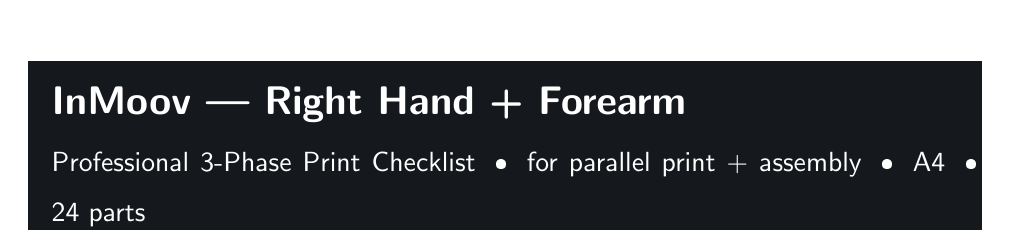
\begin{tikzpicture}
\node[anchor=west,inner sep=0pt] at (0,0){%
\colorbox{ink}{\makebox[\dimexpr\textwidth-2\fboxsep\relax][l]{%
\rule{0pt}{12mm}%
\hspace{2mm}\begin{minipage}{0.97\textwidth}
\color{white}\bfseries\Large InMoov --- Right Hand + Forearm\\[1mm]
{\normalsize\mdseries Professional 3-Phase Print Checklist \;\textbullet\; for parallel print + assembly \;\textbullet\; A4 \;\textbullet\; 24 parts}
\end{minipage}}}};
\end{tikzpicture}

\vspace{3mm}

% =================================================================
% FILAMENT & PRINTER REQUIREMENTS
% =================================================================
\noindent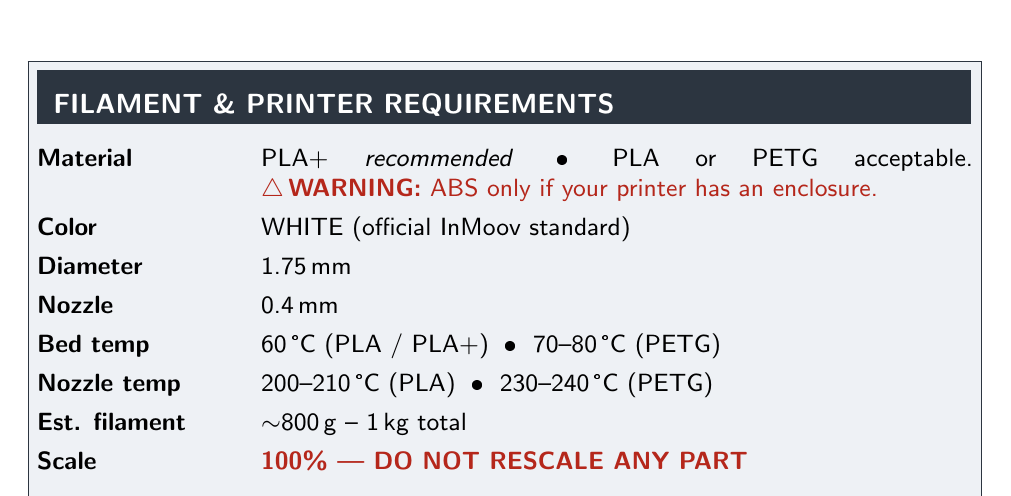
\begin{tikzpicture}
\node[anchor=west,inner sep=0pt] at (0,0){%
\fcolorbox{infohd}{infobg}{\begin{minipage}{\dimexpr\textwidth-2\fboxsep-2\fboxrule\relax}
\colorbox{infohd}{\makebox[\dimexpr\textwidth-2\fboxsep-2\fboxrule\relax][l]{\color{white}\bfseries\rule{0pt}{4.4mm}\hspace{1mm}FILAMENT \& PRINTER REQUIREMENTS}}\\[1.5mm]
\small
\begin{tabularx}{\linewidth}{@{}>{\bfseries}p{26mm} X@{}}
Material    & PLA+ \emph{recommended} \;\textbullet\; PLA or PETG acceptable. \quad\wlab\ \textcolor{warnred}{ABS only if your printer has an enclosure.}\\
Color       & WHITE (official InMoov standard)\\
Diameter    & 1.75\,mm\\
Nozzle      & 0.4\,mm\\
Bed temp    & 60\,\textdegree C (PLA / PLA+) \;\textbullet\; 70--80\,\textdegree C (PETG)\\
Nozzle temp & 200--210\,\textdegree C (PLA) \;\textbullet\; 230--240\,\textdegree C (PETG)\\
Est. filament & $\sim$800\,g -- 1\,kg total\\
Scale       & \textcolor{warnred}{\bfseries 100\% --- DO NOT RESCALE ANY PART}\\
\end{tabularx}
\vspace{1mm}
\end{minipage}}};
\end{tikzpicture}

\vspace{3mm}

% =================================================================
% CALIBRATOR FIRST
% =================================================================
\noindent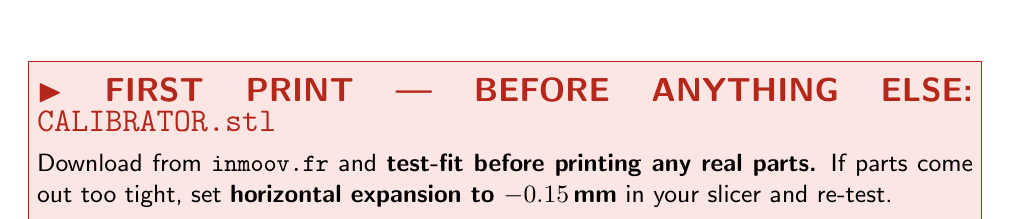
\begin{tikzpicture}
\node[anchor=west,inner sep=0pt] at (0,0){%
\fcolorbox{warnred}{warnbg}{\begin{minipage}{\dimexpr\textwidth-2\fboxsep-2\fboxrule\relax}
\vspace{1mm}
{\color{warnred}\bfseries\large $\blacktriangleright$\ FIRST PRINT --- BEFORE ANYTHING ELSE:\quad\texttt{CALIBRATOR.stl}}\\[1.2mm]
\small Download from \texttt{inmoov.fr} and \textbf{test-fit before printing any real parts.}
If parts come out too tight, set \textbf{horizontal expansion to $-0.15$\,mm} in your slicer and re-test.
\vspace{1mm}
\end{minipage}}};
\end{tikzpicture}

\clearpage

% =================================================================
% PHASE 1  (BLUE)
% =================================================================
\phasebar{p1}{p1bg}{PHASE 1 \;\textbullet\; FOREARM + WRIST BACKBONE}{PRINT FIRST}{Print these first --- start assembling the forearm immediately after}

\noindent\begin{tabularx}{\textwidth}{K >{\RaggedRight\arraybackslash}X P Q W S R}
\thead{p1}
\prow{1}{robpart2V3.stl}{0.25\,mm}{30\%}{2\,mm}{NO}{\textbf{YES}}
\pwarn{\textbf{PRINT FIRST} --- glues to \texttt{rotawrist1}. The square boss on the RotaWrist must align with the \emph{single} hole of \texttt{robpart2}. Redrill the side holes with a \textbf{6\,mm} drill. Raft = anti-warp.}
\prow{2}{robpart3V3.stl}{0.25\,mm}{30\%}{2\,mm}{NO}{\textbf{YES}}
\pnote{\nlab\ Pairs with \texttt{robpart4} --- glue these two together as a set. Raft = anti-warp.}
\prow{3}{robpart4V3.stl}{0.25\,mm}{30\%}{2\,mm}{NO}{\textbf{YES}}
\pnote{\nlab\ Pairs with \texttt{robpart3} --- glue together. The servo bed spans \texttt{robpart3/4/5}. Raft = anti-warp.}
\prow{4}{robpart5V3.stl}{0.25\,mm}{30\%}{2\,mm}{NO}{\textbf{YES}}
\pwarn{\textbf{Longest print, $\sim$7\,hrs+.} Insert two \textbf{4\,mm} bolts into the printed cavities --- heat the bolts with hot air if they don't fit. The servo bed seats here. Raft = anti-warp.}
\prow{5}{robcap3V1.stl}{0.25\,mm}{30\%}{2\,mm}{NO}{NO}
\prow{6}{rotawrist1V3.stl}{0.25\,mm}{30\%}{3\,mm}{\textbf{YES}}{NO}
\pwarn{\textbf{PRINT FIRST.} Remove support with pliers after printing. \textbf{Dry-fit against \texttt{robpart2} BEFORE gluing} --- the glue face must align perfectly. Wrong orientation = broken build. See the photo at \texttt{inmoov.fr/rotational-wrist/}.}
\prow{7}{rotawrist2.stl}{\cellcolor{warnbg}\textbf{0.15\,mm}}{50\%}{3\,mm}{NO}{NO}
\pwarn{Redrill with a \textbf{2.5\,mm} drill after printing. \tlab\ spray-paint it \textbf{BLACK} after printing (grease turns it yellow over time). Apply grease to the gear before assembly. 0.15\,mm layer = best quality for the gear teeth.}
\prow{8}{rotawrist3V2.stl}{0.25\,mm}{30\%}{3\,mm}{NO}{NO}
\pnote{\nlab\ Redrill with an \textbf{8\,mm} drill after printing. Mounts \texttt{i2\_WristLargeV2} on top.}
\prow{9}{RobServoBedV6.stl}{0.2\,mm}{30\%}{2\,mm}{NO}{NO}
\pwarn{\textbf{Dry-fit inside the \texttt{robpart3/4/5} shell before final assembly.} File the servo-bed rails if needed for fit. Secure with 2 wood screws. Spans \texttt{robpart3+4+5}, not just one section.}
\prow{10}{RobCableFrontV3.stl}{0.2\,mm}{30\%}{2\,mm}{NO}{NO}
\prow{11}{RobCableBackV3.stl}{0.2\,mm}{30\%}{2\,mm}{NO}{NO}
\bottomrule
\end{tabularx}

\vspace{1mm}
{\footnotesize\color{p1}\bfseries Phase 1: 11 prints.}

\unlocked{p1}{p1bg}{%
\begin{itemize}[leftmargin=5mm,itemsep=1.2pt,topsep=1pt]
\item Glue \texttt{robpart2} + \texttt{robpart5} together.
\item Glue \texttt{robpart3} + \texttt{robpart4} together.
\item Dry-fit \texttt{rotawrist1} on \texttt{robpart2}, then glue --- \textbf{check orientation!}
\item Insert the \textbf{MG996R} wrist servo (180\textdegree\ servo).
\item Fit the servo bed into the \texttt{robpart3/4/5} shell.
\end{itemize}}

\clearpage

% =================================================================
% PHASE 2  (GREEN)
% =================================================================
\phasebar{p2}{p2bg}{PHASE 2 \;\textbullet\; HAND CORE}{PRINT WHILE ASSEMBLING PHASE 1}{Print while assembling Phase 1 --- start finger assembly after}

\noindent\begin{tabularx}{\textwidth}{K >{\RaggedRight\arraybackslash}X P Q W S R}
\thead{p2}
\prow{12}{i2\_FingersX5V2.stl}{0.25\,mm}{30\%}{2\,mm}{NO}{NO}
\pnote{\nlab\ Contains all 5 fingers in one file ($\times$5 print). After printing, \textbf{redrill ALL finger hinge holes with a 3\,mm drill bit.} Assembly order: \textbf{Middle first}, then Index, Ring, Pinky, \textbf{Thumb last}.}
\prow{13}{i2\_FingersMoldX5V3.stl}{0.25\,mm}{30\%}{2\,mm}{NO}{NO}
\pnote{\nlab\ Mold used to cast silicone fingertips (optional). Run fishing line $\sim$30\,cm through the spring hole of each finger section.}
\prow{14}{i2\_WristLargeV2.stl}{0.25\,mm}{30\%}{2\,mm}{NO}{NO}
\pnote{\nlab\ Redrill with an \textbf{M8} drill bit. Mounts to \texttt{rotawrist3} with an M8 printed bolt + mini clamp on the bolt groove. PTFE tubes (ID\,1.5\,mm $\times$ OD\,2.5\,mm) run through the main-gear Teflon pipes.\newline
\textbf{PTFE lengths:} \;Thumb 335\,mm \;\textbullet\; Index 300\,mm \;\textbullet\; Middle 300\,mm \;\textbullet\; Ring 300\,mm \;\textbullet\; Pinky 360\,mm.}
\prow{15}{i2\_WristGearV1.stl}{\cellcolor{warnbg}\textbf{0.15\,mm}}{50\%}{3\,mm}{NO}{NO}
\pnote{\nlab\ This is the tendon \textbf{pass-through} gear, \emph{not} the rotation gear. PTFE tubes run through this gear's Teflon-pipe holes. 0.15\,mm = best quality (gear part).}
\prow{16}{i2\_PulleyX5V1.stl}{\cellcolor{warnbg}\textbf{0.15\,mm}}{50\%}{3\,mm}{NO}{NO}
\pnote{\nlab\ Hand-side pulley (redirects the tendon at the hand). \textbf{DIFFERENT from \texttt{servo-pulleyX5} --- both are required.} 0.15\,mm = best quality.}
\prow{17}{RobRingV3.stl}{0.2\,mm}{30\%}{2\,mm}{NO}{NO}
\prow{18}{TensionerRightV1.stl}{0.2\,mm}{30\%}{2\,mm}{NO}{NO}
\pwarn{\textbf{RIGHT-hand version only --- do NOT substitute a Left version.} Screws onto the servo bed.}
\prow{19}{servo-pulleyX5.stl}{\cellcolor{warnbg}\textbf{0.15\,mm}}{50\%}{3\,mm}{NO}{NO}
\pnote{\nlab\ Mounts on the servo output horns inside the servo bed ($\times$5, one per servo). Redrill with a \textbf{2\,mm} drill after printing. \textbf{DIFFERENT from \texttt{i2\_PulleyX5V1} --- both are required.} 0.15\,mm = best quality (takes direct servo load).}
\bottomrule
\end{tabularx}

\vspace{1mm}
{\footnotesize\color{p2}\bfseries Phase 2: 8 prints.}

\unlocked{p2}{p2bg}{%
\begin{itemize}[leftmargin=5mm,itemsep=1.2pt,topsep=1pt]
\item Mount \texttt{i2\_WristLargeV2} to \texttt{rotawrist3} with the M8 bolt; set the mini clamp on the bolt groove.
\item Assemble the fingers to WristLarge with \textbf{M3$\times$16\,mm} screws (order: Middle, Index, Ring, Pinky, Thumb).
\item Install 5$\times$ \textbf{MG995} finger servos in the servo bed --- \textbf{set each servo to 150\textdegree\ before mounting.}
\item Run PTFE tubes through the WristGear Teflon pipes.
\item Run PTFE tubes through the servo-bed holes to the servo shafts.
\end{itemize}}

\clearpage

% =================================================================
% PHASE 3  (ORANGE)
% =================================================================
\phasebar{p3}{p3bg}{PHASE 3 \;\textbullet\; COVERS + TIPS}{PRINT LAST}{Hand is functional without these --- print while doing Phase 2 assembly}

\noindent\begin{tabularx}{\textwidth}{K >{\RaggedRight\arraybackslash}X P Q W S R}
\thead{p3}
\prow{20}{i2\_CoverFingerV3.stl}{0.25\,mm}{30\%}{2\,mm}{\textbf{YES}}{If needed}
\pnote{\tlab\ Print \textbf{STANDING UPRIGHT} for the best surface result (not flat).}
\prow{21}{i2\_FingersTipX5V2.stl}{0.25\,mm}{30\%}{2\,mm}{\textbf{YES}}{If needed}
\pnote{\nlab\ Glue the tips onto the finger sections \textbf{AFTER} assembly. Do \emph{not} glue them on before assembly --- they look wrong in the closed position.}
\prow{22}{i2\_HandCoverV1.stl}{0.25\,mm}{30\%}{2\,mm}{\textbf{YES}}{If needed}
\pnote{\nlab\ Before screwing, tap the holes with an \textbf{M3 tap} for M3$\times$16\,mm screws.}
\prow{23}{i2\_PalmCoverV2.stl}{0.25\,mm}{30\%}{2\,mm}{\textbf{YES}}{If needed}
\pwarn{When screwing the palm cover, \textbf{set the ribbons neatly into the grooves. AVOID pinching ribbons --- this kills the electronics.}}
\prow{24}{i2\_Adapter1109MG.stl}{0.25\,mm}{30\%}{2\,mm}{\textbf{YES}}{If needed}
\pnote{\nlab\ Servo adapter for the 1109MG servo type.}
\bottomrule
\end{tabularx}

\vspace{1mm}
{\footnotesize\color{p3!88!black}\bfseries Phase 3: 5 prints.}

\unlocked{p3}{p3bg}{%
\begin{itemize}[leftmargin=5mm,itemsep=1.2pt,topsep=1pt]
\item Tap all cover holes with the M3 tap.
\item Mount the HandCover and PalmCover.
\item Route all ribbon cables neatly into the PalmCover grooves.
\item Glue the FingerTips onto the finger sections.
\item Final tensioning of the fishing-line tendons.
\end{itemize}}

\vspace{3.5mm}

% =================================================================
% TOTALS / SIGN-OFF
% =================================================================
\noindent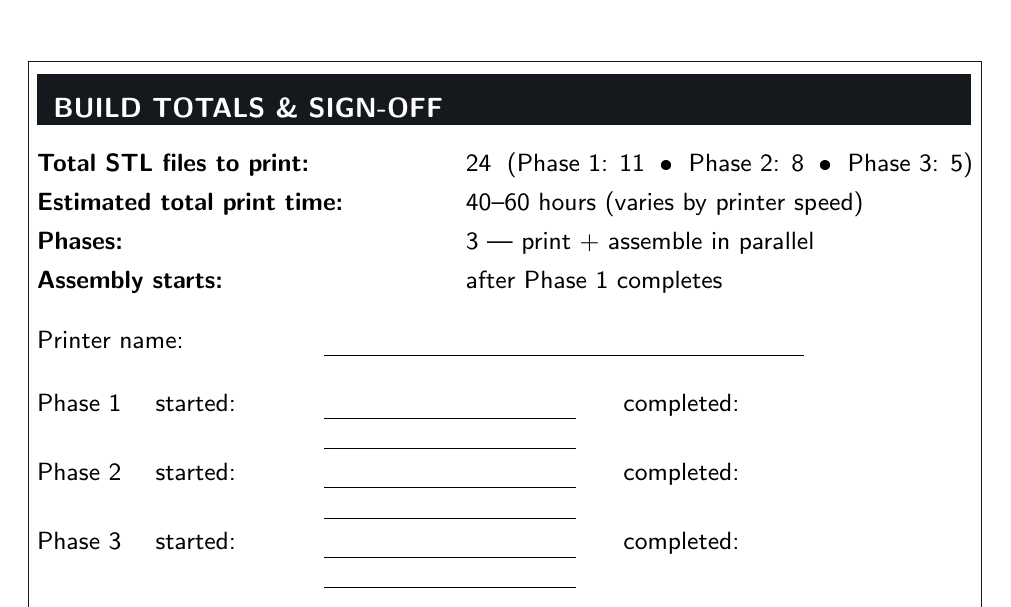
\begin{tikzpicture}
\node[anchor=west,inner sep=0pt] at (0,0){%
\fcolorbox{ink}{white}{\begin{minipage}{\dimexpr\textwidth-2\fboxsep-2\fboxrule\relax}
\vspace{0.5mm}
\colorbox{ink}{\makebox[\dimexpr\textwidth-2\fboxsep-2\fboxrule\relax][l]{\color{white}\bfseries\rule{0pt}{4.4mm}\hspace{1mm}BUILD TOTALS \& SIGN-OFF}}\\[2mm]
\small
\begin{tabularx}{\linewidth}{@{}>{\bfseries}p{52mm} X@{}}
Total STL files to print: & 24 \;(Phase 1: 11 \;\textbullet\; Phase 2: 8 \;\textbullet\; Phase 3: 5)\\
Estimated total print time: & 40--60 hours (varies by printer speed)\\
Phases: & 3 --- print + assemble in parallel\\
Assembly starts: & after Phase 1 completes\\
\end{tabularx}
\vspace{2mm}

\begin{tabularx}{\linewidth}{@{}p{34mm} X@{}}
Printer name: & \rule[-1mm]{0.74\linewidth}{0.4pt}\\[3mm]
Phase 1 \quad started: & \rule[-1mm]{32mm}{0.4pt}\hspace{6mm}completed: \rule[-1mm]{32mm}{0.4pt}\\[3mm]
Phase 2 \quad started: & \rule[-1mm]{32mm}{0.4pt}\hspace{6mm}completed: \rule[-1mm]{32mm}{0.4pt}\\[3mm]
Phase 3 \quad started: & \rule[-1mm]{32mm}{0.4pt}\hspace{6mm}completed: \rule[-1mm]{32mm}{0.4pt}\\[1mm]
\end{tabularx}
\vspace{1mm}
\end{minipage}}};
\end{tikzpicture}

\clearpage

% =================================================================
% TOOLS NEEDED
% =================================================================
\noindent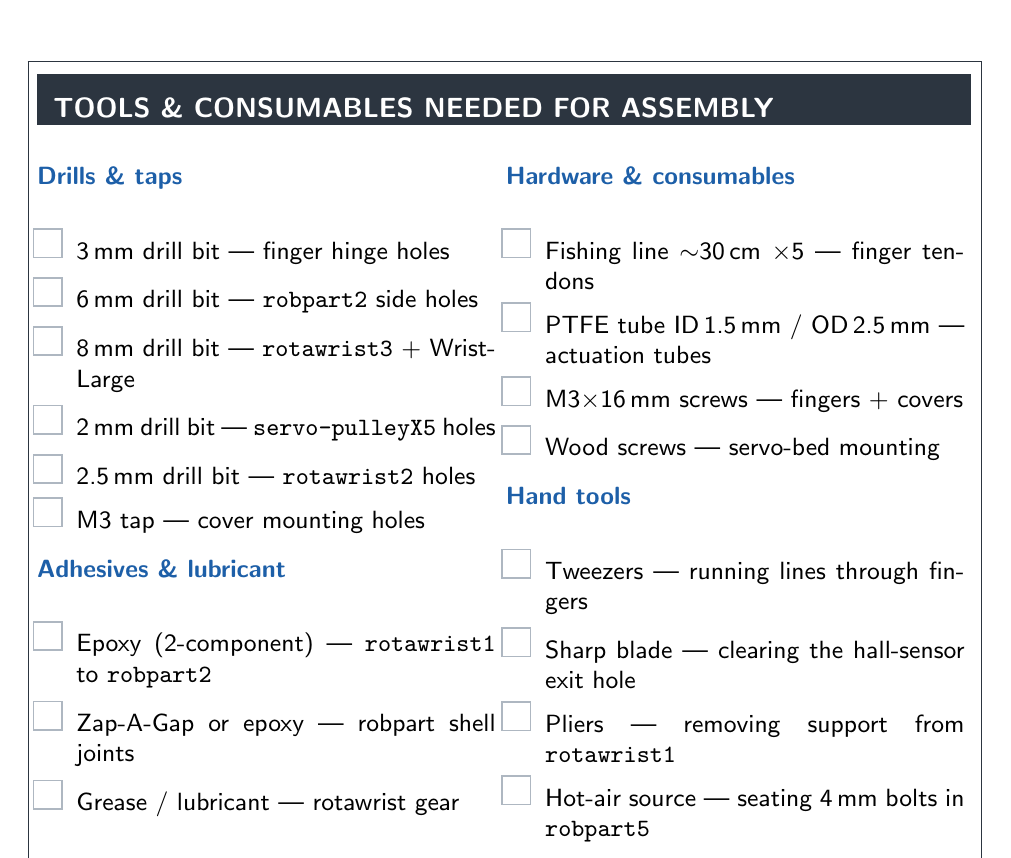
\begin{tikzpicture}
\node[anchor=west,inner sep=0pt] at (0,0){%
\fcolorbox{infohd}{white}{\begin{minipage}{\dimexpr\textwidth-2\fboxsep-2\fboxrule\relax}
\vspace{0.5mm}
\colorbox{infohd}{\makebox[\dimexpr\textwidth-2\fboxsep-2\fboxrule\relax][l]{\color{white}\bfseries\rule{0pt}{4.4mm}\hspace{1mm}TOOLS \& CONSUMABLES NEEDED FOR ASSEMBLY}}\\[2.5mm]
\small
\begin{minipage}[t]{0.49\linewidth}
{\color{p1}\bfseries Drills \& taps}\\[1mm]
\begin{itemize}[leftmargin=5mm,itemsep=1.6pt,topsep=1pt,label=\cbox]
\item 3\,mm drill bit --- finger hinge holes
\item 6\,mm drill bit --- \texttt{robpart2} side holes
\item 8\,mm drill bit --- \texttt{rotawrist3} + WristLarge
\item 2\,mm drill bit --- \texttt{servo-pulleyX5} holes
\item 2.5\,mm drill bit --- \texttt{rotawrist2} holes
\item M3 tap --- cover mounting holes
\end{itemize}
\vspace{2mm}
{\color{p1}\bfseries Adhesives \& lubricant}\\[1mm]
\begin{itemize}[leftmargin=5mm,itemsep=1.6pt,topsep=1pt,label=\cbox]
\item Epoxy (2-component) --- \texttt{rotawrist1} to \texttt{robpart2}
\item Zap-A-Gap or epoxy --- robpart shell joints
\item Grease / lubricant --- rotawrist gear
\end{itemize}
\end{minipage}\hfill
\begin{minipage}[t]{0.49\linewidth}
{\color{p1}\bfseries Hardware \& consumables}\\[1mm]
\begin{itemize}[leftmargin=5mm,itemsep=1.6pt,topsep=1pt,label=\cbox]
\item Fishing line $\sim$30\,cm $\times$5 --- finger tendons
\item PTFE tube ID\,1.5\,mm / OD\,2.5\,mm --- actuation tubes
\item M3$\times$16\,mm screws --- fingers + covers
\item Wood screws --- servo-bed mounting
\end{itemize}
\vspace{2mm}
{\color{p1}\bfseries Hand tools}\\[1mm]
\begin{itemize}[leftmargin=5mm,itemsep=1.6pt,topsep=1pt,label=\cbox]
\item Tweezers --- running lines through fingers
\item Sharp blade --- clearing the hall-sensor exit hole
\item Pliers --- removing support from \texttt{rotawrist1}
\item Hot-air source --- seating 4\,mm bolts in \texttt{robpart5}
\end{itemize}
\end{minipage}
\vspace{1.5mm}
\end{minipage}}};
\end{tikzpicture}

\vspace{4mm}

{\footnotesize\color{ink!70}Settings sourced from \texttt{inmoov.fr/hand-and-forarm/}, \texttt{inmoov.fr/hand-i2/}, \texttt{inmoov.fr/rotational-wrist/} and community builders. Print-time estimate assumes $\sim$50--60\,mm/s; faster/slower printers will differ. Verify all redrill/tap operations on a test print before committing to a full set.}

\end{document}
